\documentclass[iicol,sn-basic]{sn-jnl}

\usepackage{amsmath}
\usepackage{amssymb}
\usepackage{amsthm}
\usepackage{hyperref}
\usepackage{booktabs}
\usepackage{soul}
\usepackage{bm}
\usepackage{subcaption}
\usepackage{wrapfig}
\usepackage{anysize}
\usepackage{cancel}
\marginsize{1in}{1in}{1in}{1in}

\newtheorem{prop}{Proposition}
\DeclareMathOperator{\tr}{Tr}
\DeclareMathOperator*{\argmin}{arg\,min}
\DeclareMathOperator*{\argmax}{arg\,max}
\newcommand{\bigmid}{\,\middle\vert\,}

\newcommand{\findcite}{\textcolor{red}{[Find Citation]}}
\newcommand{\needcite}{\findcite}
\newcommand{\Chi}{\mbox{\Large$\chi$}}
\newcommand{\mathcolorbox}[2]{\colorbox{#1}{$\displaystyle #2$}}

\newcommand{\norm}[1]{\left\lVert #1 \right\rVert}
\newcommand{\inorm}[1]{\norm{#1}_{\infty}}
\newcommand{\pnorm}[2]{\norm{#1}_{#2}}
\newcommand{\prob}[1]{\text{Pr}\left[#1\right]}
\newcommand{\expect}[1]{\text{E}\left[#1\right]}

\jyear{2023}
\theoremstyle{thmstyleone}

\raggedbottom

\begin{document}

\title[~\hspace{6.75in}BNP inference for multivariate PoT]{Bayesian non-parametric inference for multivariate peaks-over-threshold models}

\author*{\fnm{Peter} \sur{Trubey}}\email{ptrubey@ucsc.edu}
\author{\fnm{Bruno} \sur{Sans\'{o}}}\email{bruno@soe.ucsc.edu}

\affil{\orgdiv{Department of Statistics}, \orgname{University of California Santa Cruz},
\orgaddress{\street{1156 High Street}, \city{Santa Cruz},\postcode{95064}, \state{CA}, \country{USA}}}

\abstract{\bf{\colorbox{red}{Note: Assume tables, algorithms and figures have changed.  Highlighting changes}}

\bf{\colorbox{red}{in these environments is not straightforward.}}

We consider a constructive definition of the multivariate Pareto that 
factorizes the random vector into a radial component and an independent angular 
component; The former following a univariate Pareto distribution, and the latter 
defined on the surface of the positive orthant of the infinity norm unit hypercube.  In this 
paper, we  propose a method for inferring the distribution of the angular 
component.  We identify its support as the limit of the positive orthant of the 
unit $p$--norm spheres, and introduce a projected gamma family of distributions 
defined \st{as}\hl{through} the \st{projec}\hl{normaliza}tion of a vector of independent gamma random variables \st{on}to 
the $p$--norm sphere.  This family serves as a building block for a flexible 
family of distributions obtained as a Dirichlet process mixture of projected 
gammas.  For model assessment, we discuss scoring methods appropriate to 
distributions on the unit hypercube.  In particular, working with the energy 
score criterion, we develop a kernel metric that produces a proper scoring rule, 
and present a simulation study to compare different modeling choices using the 
proposed scoring rules.  Finally we apply our approach to describe the 
dependence structure of the extreme values of the magnitude of the integrated 
vapor transport (IVT), data describing the flow of atmospheric moisture along 
the coast of California for the years of 1979 through 2020.  We find clear but 
heterogeneous geographical dependence.}
\keywords{Multivariate extremes, Peak over threshold models, Bayesian non-parametric models, Dirichlet process mixtures}

\maketitle

%--------content

\section{Introduction}

The statistical analysis of extreme values focuses on inference for rare events that correspond to the tails of probability distributions. As such, it is a key ingredient in the risk assessment of phenomena that can have strong societal impacts like floods, heat waves, high concentration of pollutants, crashes in the financial markets, among others. The fundamental challenge of extreme value theory (EVT) is to use information, collected over limited periods of time, to extrapolate to long time horizons. This sets EVT apart from most of statistical inference, where the focus is on the bulk of the distribution. Extrapolation to the tails of the distributions is possible thanks to theoretical results that give asymptotic descriptions of the probability distributions of extreme values.

Inferential methods for the extreme values of univariate observations are well established and software is widely available \cite[see, for example,][]{coles2001}. For variables in one dimension the application of EVT methods considers the asymptotic distribution of either the maxima calculated for regular blocks of data, or the values that exceed a certain threshold. The former leads to a Generalized Extreme Value (GEV) distribution, that depends on three parameters. The latter leads to a Generalized Pareto (GP) distribution, that depends on a shape and a scale parameter.  Likelihood-based approaches to inference can be readily implemented in both cases. In the multivariate case the GEV theory is well developed \citep[see, for example][]{dehaan2006}, but the inferential problem is \st{more} complicated\st{, as} \hl{by the fact that} there is no parametric representation of the GEV. This problem is inherited by the peaks over threshold (PoT) approach and compounded by the fact that there is no unique definition of an exceedance of a multivariate threshold, as there is an obvious dependence on the norm that is used to measure the size of a vector.

During the last decade or so, much work has been done in the exploration of the definition and properties
of an appropriate generalization of the univariate GP distribution to a multivariate setting.  To mention
some of the papers on the topic, the work of \citep{rootzen2006} defines the generalized Pareto distribution,
with further analysis on these classes of distributions presented in \cite{falk2008} and \cite{michel2008}.  
A recent review of the state of the art in multivariate peaks over threshold modelling using generalized 
Pareto is provided in \cite{rootzen2018} while \cite{RoSeWa2018a} provides insight on the theoretical 
properties of possible parametrizations. These are use in \cite{KiRoSeWa2019} for likelihood-based models 
for PoT estimation. A frequently used method for describing the dependence in multivariate distributions is
to use a copula. \cite{renard2007}, and \cite{falk2019} provide successful examples of this approach in an 
EVT framework. \cite{ferreira2014} presents a constructive definition of the Pareto process, that generalizes
the GP to an infinite dimensional setting. It consists of decomposing the process into independent radial and 
angular components. Such an approach can be used in the finite dimensional case, where the angular component 
contains the information pertaining to the dependence structure of the random vector. Based on this definition, 
we present a novel approach for modelling  the angular component with families of distributions that provide 
flexibility and can be applied in a moderately large dimensional setting.  Our focus on the angular measure is 
similar to that in \hl{\mbox{\cite{boldi2007}}}, \cite{SaNa2014} and \cite{HaCaCh2017}, that consider Bayesian 
non-parametric approaches. Yet, our approach \hl{differs in that it is established in the peaks-over-threshold 
regime, and }avoids the problem of dealing with the so called moment constraint by considering a constructive 
definition of the multivariate GP, based on the infinity norm. \hl{The approach proposed in this paper adds to 
the growing literature on Bayesian models for multivariate extreme value analysis (see, for example, 
\mbox{\cite{boldi2007}}, \mbox{\cite{guillotte2011}}, \mbox{\cite{SaNa2014}}, \mbox{\cite{hanson2017}}), providing a model that has strong computational advantages due its structural simplicitly, achieves flexibility using a mixture model, imposes no moment constraints, and scales well to moderately large dimensions.}

The remainder of this paper is outlined as follows. Section~\ref{sec:multivariatepot} comprises a brief review of multivariate PoT, detailing the separation of the radial measure from the angular measure. Section~\ref{sec:methodology} details our approach for estimating the angular measure, based on projecting an arbitrary distribution supported in ${\mathbb R}_+^d$ onto unit hyper-spheres defined \st{for}\hl{by} $p$-norms. Section~\ref{sec:evaluation} develops criteria for model selection in the support of the angular measure.  Section~\ref{sec:results} explores the efficacy of the proposed approach on a set of simulated data, and, acknowledging the relevance of extreme value theory to climatological events~\citep{jentsch2007,vousdoukas2018,li2019}, estimates the extremal dependence structure for a measure of water vapor flow in the atmosphere, used for identifying atmospheric rivers.  Finally, Section~\ref{sec:conclusion} presents our conclusions and discussion.

Throughout the paper, we adopt the operators $\wedge$ to denote minima, and the $\vee$ to denote maxima.  Thus $\wedge_i s_i = \min_i s_i$, and $\vee_i s_i = \max_i s_i$.  These operators can also be applied component-wise between vectors, such as $\bm{a}\wedge\bm{b} = (a_1\wedge b_1, a_2\wedge b_2,\ldots)$.  We use uppercase to indicate random variables, lowercase to indicate points, and bold-face to indicate vectors or matrices thereof.

\section{A multivariate PoT model\label{sec:multivariatepot}}
To develop a multivariate PoT model for extreme values consider a $d$-dimensional random vector $\bm{W} = (W_1, \ldots ,W_d)$ with cumulative distribution $F$. Following \cite{RoSeWa2018a}, assume that there exists sequences of vectors $\bm{a}_n$ and $\bm{b}_n$, and a $d$-variate distribution $G$ such that $\lim_{n\rightarrow\infty} F^n(\bm{a}_n \bm{w} + \bm{b}_n) = G(\bm{w})$. $G$ is a $d$-variate generalized extreme value distribution. It follows that
\begin{equation*}
\begin{aligned}
\lim\limits_{n\rightarrow\infty} &\prob{\bm{a}^{-1}_n (\bm{W} - \bm{b}_n)
\leq \bm{w} \mid \bm{W} \not\leq \bm{b}_n)} \\
&\hspace{0.5cm}= \frac{\log G(\bm{w} \wedge \bm{0})
- \log G(\bm{w}) }{\log G(\bm{0})} = H(\bm{w}).
\end{aligned}
\end{equation*}
$H$ is \st{the}\hl{a} multivariate Pareto distribution\hl{, and corresponds to a joint distribution conditional on exceeding a multivariate threshold. In addition to a copula function, $H$ depends on two $d$-dimensional vectors of parameters that we denote as $\bm{\xi}$ for the shapes and $\bm{\sigma}$ for the scales}. \cite{RoSeWa2018a} provide a number of stochastic representations for $H$. In particular\hl{, denote as $Z$ a random variable with distribution $H$ where $\bm{\xi}= 1$ and $\bm{\sigma} = 0$.  Then,} Remark 1 justifies the representation \st{given } in \cite{ferreira2014}, \st{consisting of taking $\bm{W}$, in the limit, as $\bm{W} = \bm{V}R$} \hl{giving $\bm{Z} = \bm{V}R$} where $R$ and $\bm{V}$ are independent. \st{$R = ||\bm{W}||_\infty$}\hl{$R = \|\bm{Z}\|_\infty$} is distributed as a standard Pareto random variable, and \st{$\bm{V} = \bm{W}/||\bm{W}||_\infty$}\hl{$\bm{V} = \bm{Z}/\|\bm{Z}\|_\infty$} is a random vector in $\mathbb{S}_{\infty}^{d-1}$, the positive orthant of the unit sphere \st{in infinite}\hl{under $\mathcal{L}_{\infty}$} norm, with distribution $\Phi$.  \hl{This representation is central to the methods proposed in this paper.  }$R$ and $\bm{V}$ are referred\hl{ to}, respectively, as the {\em radial} and {\em angular} components of $H$. The angular measure controls the dependence  structure of \st{ $\bm{W}$} \hl{$\bm{Z}$}  in the tails. In view of this, to obtain a  PoT model we seek a flexible model for the distribution of $\bm{V} \in {\mathbb S}_{\infty}^{d-1}$.

\hl{The approach considered in \mbox{\cite{rootzen2018}} focuses on the limiting conditional distribution $H$. An alternative approach consists of assuming that regular variation \mbox{\cite[see, for example,][]{resnick2008extreme}} holds for the limiting distribution of $\bm{W}$, implying}
\[
\mathcolorbox{yellow}{\lim\limits_{n\rightarrow\infty} n \prob{n^{-1} \bm{W}\in A} = \mu(A),}
\]
\hl{where $\mu$ is termed the exponent measure. $\mu$ has the homogeneity property $\mu(tA) = t^{-1}\mu(A)$. Letting $\rho = \|W\|_p, p>0$ and $\bm{\theta} = \bm{W}/\rho$, define  $\Psi(B) = \mu(\{\bm{w} : \rho>1, \bm{\theta} \in B\})$, which is referred to as the angular measure. After some manipulations, we obtain that}
\begin{equation}
\label{exponent-mu}
\mathcolorbox{yellow}{\lim\limits_{r\rightarrow\infty}\text{Pr}\left[\bm{\theta}\in A \rvert \rho>r\right] =\frac{\Psi(A)}{\Psi({\mathbb S}_p^{d-1})}.}
\end{equation}
\hl{Thus, a model for the exponent measure induces a model for the limiting distribution conditional on the observations being above a threshold defined with respect to their $p$-norm. The constraint that all marginals of $\mu$ correspond to a standard Pareto distribution leads to the so called moment constraints on $\Psi$. Inference for the limiting distribution of the exceedances needs to account for the normalizing constant in Equation~(\mbox{\ref{exponent-mu}}), as well the moment constraints. In addition, the moment constraints can impose unrealistic symmetries in the data distribution}

\section{Estimation of the angular measure\label{sec:methodology}}

Our approach to estimating the PoT distribution considers two steps: First we estimate the shape and scale parameters for the multivariate Pareto distribution, using the univariate marginals; Then we focus on the dependence structure in extreme regions by proposing a flexible model for the distribution of $\bm{V}$. Consider a collection of observations  $\bm{w}_i \in {\mathbb R}^d, i = 1, \ldots, n$ that exhibit extreme behavior.  We start by setting a large threshold $b_{t,\ell}$ for the  $\ell$-th marginal, $\ell = 1, \ldots,d$. Then, the distribution of the observations for the $\ell$-th component, conditional on exceeding the threshold, can be approximated as $1 - (1 + \xi_\ell   (w_{i\ell} - b_{t,\ell})/\sigma_\ell)_+^{1/\xi_\ell}$, where $(\cdot)_+$ indicates the positive part function.  We proceed by setting a threshold equal to the empirical $(1-1/t)$-quantile. Thus $b_{t,l}  = \hat{F}^{-1}_{\ell}(1 - 1/t)$.  We then use the approximate exceedance distribution to estimate $\xi_\ell$ and $\sigma_\ell$, for each $\ell$, using likelihood based methods. Then, in order to estimate the angular distribution, we use those estimates to standardize each of the marginals. The standardization yields
\begin{equation}
\label{eqn:standardization}
z_{i\ell} = \left(1 + \xi_{\ell}\frac{w_{i\ell} - b_{t,\ell}}{a_{\ell}}\right)_{+}^{1/\xi_{\ell}}\; .
\end{equation}
Note that $z_{i\ell}> 1$ implies that $w_{i\ell} > b_{t,\ell}$, meaning that the observation $\bm{w}_i$ is extreme in the $\ell$-th dimension. Thus, $r_i = \|\bm{z}_i\|_\infty > 1$ implies that at least one dimension has an extreme observation, and corresponds to a very extreme observation when $t$ is large. We focus on  the observations that are such that $r_i > 1$. These provide a sub-sample of the stardardized original sample. We define $\bm{v}_i = \bm{z}_i /r_i \in  \mathbb{S}_{\infty}^{d-1}$. These vectors are used for  the estimation of $\Phi$.

\subsection{Projected gamma family\label{subsec:projgamma}}
The $\mathcal{L}_p$-norm, for $p>0$ is  defined as
\begin{equation*}
\lVert \bm{x} \rVert_p =
\left({\textstyle\sum}_{\ell = 1}^d \lvert s_{\ell}\rvert^p\right)^{\frac{1}{p}},
\end{equation*}
The absolute and Euclidean norms are obtained for $p=1$ and $p=2$ respectively, and the $\mathcal{L}_{\infty}$ norm can be obtained as a limit,
\begin{equation*}
\| \bm{s} \|_{\infty}
= \lim\limits_{p\to\infty} \| \bm{s} \|
= \underset{\ell = 1}{\overset{d}{\bigvee}}s_{\ell}.
\end{equation*}

\st{To define an angular measure,  we are interested in the direction of vectors in ${\mathbb R}_{+}^d$, thus, we project them onto}
\begin{equation*}
{\mathbb S}_{p}^{d-1} = \left\lbrace \bm{s} : \bm{s} \in {\mathbb R}_{+}^{d}, \lVert \bm{s}\rVert_{p} = 1\right\rbrace,
\end{equation*}
\st{the $\mathcal{L}_p$-norm unit hypersphere.  Given $\bm{x}\in {\mathbb R}^d_+$ the projection onto ${\mathbb S}_{p}^{d-1}$ is given as $\bm{y} = \bm{x} / \lVert \bm{x}\rVert_p \in {\mathbb S}_{p}^{d-1}$. Observations on one hypersphere can be projected without loss of information onto another by dividing by the defining norm of the target hypersphere. In fact, for finite $p$, letting $y_d = \left(1 - {\textstyle\sum}_{\ell = 1}^{d-1}y_{\ell}^p\right)^{\frac{1}{p}}$, the transformation}

\hl{To obtain a distribution on ${\mathbb S}_{p}^{d-1}=\{\bm{s} : \bm{s} \in {\mathbb R}_{+}^{d}, \| \bm{s}\|_{p} = 1\}$ we start with a vector in $\bm{x} \in {\mathbb R}^d_+$, and normalize it to obtain $\bm{y} = \bm{x}/\|\bm{x}\|_p \in {\mathbb S}_p^{d-1}$. A natural  distribution to consider in ${\mathbb R}^d_+$ is given by a product of independent univariate Gamma distributions. Let $\bm{ X} \sim \prod_{\ell = 1}^d\text{Ga}\left(X_{\ell}\mid\alpha_{\ell},\beta_{\ell}\right)$, $\alpha_\ell$ and $\beta_\ell$ are the shape and scale parameters, respectively. For any finite $p>0$, letting $ y_d = (1 - {\textstyle\sum}_{\ell = 1}^{d-1}y_{\ell}^p)^{1/p}$, the transformation}
\begin{equation}
\label{eqn:pnormt}
\begin{aligned}
T(x_1,\ldots,x_d) &= \left(\pnorm{\bm{x}}{p}, \frac{x_1}{\pnorm{\bm{x}}{p}}, \ldots , \frac{x_{d-1}}{\pnorm{\bm{x}}{p}}\right) \\
&= (r,y_1,\ldots,y_{d-1})
\end{aligned}
\end{equation}
is invertible with
\begin{equation}
\label{eqn:pnormtinv}
\begin{aligned}
&\hspace{-0.5cm}T^{-1}\left(r,y_1,\ldots,y_{d-1}\right)\\
& = \left(ry_1,\ldots,ry_{d-1}, r\left(1 - {\textstyle\sum}_{\ell = 1}^{d-1}y_{\ell}^p\right)^{\frac{1}{p}}\right).
\end{aligned}
\end{equation}
The Jacobian of the transformation takes the form
\begin{equation}
\label{eqn:pnormjac}
\begin{aligned}
r^{d-1}\left[\left(1 - {\textstyle\sum}_{\ell = 1}^{d-1}y_{\ell}^p\right)^{\frac{1}{p}} \right. & \\
&\hspace{-2cm}+ \left. {\textstyle\sum}_{\ell = 1}^{d-1}y_{\ell}^p\left(1 - {\textstyle\sum}_{l=1}^{d-1} y_{\ell}^p\right)^{\frac{1}{p} - 1}\right].
\end{aligned}
\end{equation}
\st{Equations (\mbox{\ref{eqn:pnormt}}) -- (\mbox{\ref{eqn:pnormjac}}) can be used to define a density on ${\mathbb R}^d_+$, and then obtain a density on ${\mathbb S}_{p}^{d-1}$, for any finite $p>0$.}

\st{A natural  distribution to consider in ${\mathbb R}^d_+$ is given by a product of independent univariate Gamma distributions. Let $\bm{ X} \sim \prod_{\ell = 1}^d\text{Ga}\left(X_{\ell}\mid\alpha_{\ell},\beta_{\ell}\right)$, $\alpha_\ell$ and $\beta_\ell$ are the shape and scale parameters, respectively.}
\hl{The normalization provided by $T$ maps a vector in ${\mathbb R}_+^d$ onto
${\mathbb S}_p^{d-1} $. With a slight abuse of terminology we refer to it as a
projection.} Using Equations (\ref{eqn:pnormt}) -- (\ref{eqn:pnormjac}) we have the joint density
\begin{equation}
\label{joint}
\begin{aligned}
f(r,\bm{ y}) = &\prod_{\ell = 1}^{d}
\left[\frac{\beta_{\ell}^{\alpha_{\ell}}}{\Gamma(\alpha_{\ell})}(ry_{\ell})^{\alpha_{\ell} - 1}
\exp\lbrace-\beta_{\ell}ry_{\ell}\rbrace\right] \\
&\hspace{0.5cm}\times r^{d-1}\left[y_d +
{\textstyle \sum}_{\ell = 1}^{d-1}y_{\ell}^p y_d^{1 - p}\right].
\end{aligned}
\end{equation}
Integrating out $r$ yields the resulting \emph{Projected Gamma} density
\begin{equation}
\label{eqn:projgamma}
\begin{aligned}
\text{PG}(\bm{ y}\mid\bm{ \alpha},\bm{ \beta}) &=
\prod_{\ell = 1}^d\left[\frac{\beta_{\ell}^{\alpha_{\ell}}}{\Gamma(\alpha_{\ell})}
y_{\ell}^{\alpha_{\ell} - 1}\right]\\
&\hspace{0.5cm}\times \left[y_d +
{\textstyle \sum}_{\ell = 1}^{d-1}y_{\ell}^p y_d^{1 - p}\right]\\
&\hspace{0.5cm}\times \frac{\Gamma({\textstyle\sum}_{\ell = 1}^d\alpha_{\ell})}{\left({\textstyle\sum}_{\ell = 1}^d
\beta_{\ell}y_{\ell}\right)^{{\scriptstyle\sum_{\ell = 1}^d \alpha_{\ell}}}},
\end{aligned}
\end{equation}
defined for $\bm{y}\in {\mathbb S}_p^{d-1}$, and for any \hl{finite }$p>0$. To avoid identifiability problems when estimating the shape and scale parameters, we set $\beta_1 = 1$.  \cite{nunez2019} obtain the density in Equation (\ref{eqn:projgamma}) for $p=2$ as a multivariate distribution for directional data, using spherical coordinates.  For $\bm{ y}\in {\mathbb S}_1^{d-1}$, and $\beta_{\ell} = \beta$ for all $\ell$, the density in Equation~(\ref{eqn:projgamma}) corresponds to that of a Dirichlet distribution.


The projected gamma family is simple to specify and has very tractable computational properties. Thus, we use it as a building block for the angular measure $\Phi$ models. To build a flexible family of distributions in ${\mathbb S}_p^{d-1}$ we consider mixtures of projected gamma densities defined as
\begin{equation} \label{eqn:PGmix}
f(\bm{y}) = \int_\Theta \mathcal{PG}(\bm{y}\mid \bm{\theta}) dG(\bm{\theta}),
\end{equation}
where $\bm{\theta} = (\bm{\alpha}, \bm{\beta})$. Following a Bayesian non-parametric approach \citep{Ferguson74,Antoniak1974}\hl{\mbox{\citep{muller2015}}}, we assume that $G$ is drawn from a random measure. In particular, assuming a Dirichlet process prior for $G$, we have a hierarchical formulation of the mixture model that, for a vector of observations $\bm{y}_i$, is given by
\begin{equation}\label{eqn:dppg}
\begin{aligned}
\bm{y}_i &\sim \text{PG}(\bm{y}_i\mid \bm{\theta}_i)\\
\bm{\theta}_i &\sim G
\end{aligned}
~\hspace{1cm}
\begin{aligned}
G &\sim \mathcal{DP}(\eta, G_0),
\end{aligned}
\end{equation}
where $\mathcal{DP}$ denotes a Dirichlet process, $\eta$ is the precision parameter, and $G_0$ is the centering distribution.

Unfortunately, in the limit when $p\rightarrow \infty$, the \st{projection}\hl{normalizing} transformation is not differentiable. Thus, a closed form expression like Equation (\ref{eqn:projgamma}) for the projected gamma density on ${\mathbb S}_\infty^{d-1}$ is not available. Instead, we observe that for a sufficiently large $p$, $\mathbb{S}_p^{d-1}$ will approach $\mathbb{S}_{\infty}^{d-1}$.  With that in mind, our strategy consists of describing the angular distribution $\Phi$ using a sample based approach with the following steps: (i) Apply the transformation in Equation (\ref{eqn:standardization}) to the original data; (ii) Obtain the subsample of the standardized observations that satisfy $R>1$; (iii) Take a finite $p$ and project the observations onto ${\mathbb S}_p^{d-1}$; (iv) Fit the model in Equation (\ref{eqn:PGmix}) to the resulting data and obtain samples from the fitted model; (v) Project the resulting samples onto ${\mathbb S}_\infty^{d-1}$. For step (iv) we use a Bayesian approach that is implemented using a purposely developed Markov chain Monte Carlo sampler described in the next section.
\begin{figure}[ht]
\centering
\caption{The positive orthant of the $p$-norm sphere.}
\begin{subfigure}[b]{0.4\textwidth}
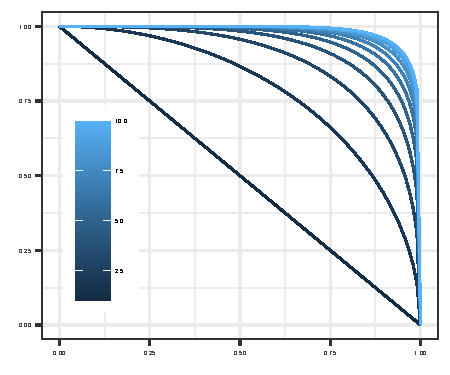
\includegraphics[width=\textwidth]{./images/p_sphere}
\caption{${\mathbb S}_p^1$ for $p = 1,\ldots, 10$\label{fig:psphere}}
\end{subfigure}
%
\begin{subfigure}[b]{0.4\textwidth}
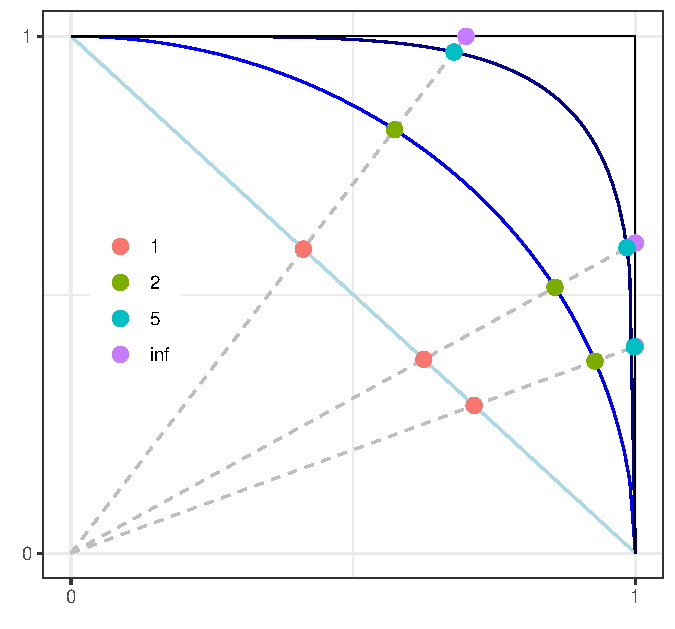
\includegraphics[width=\textwidth]{./images/p_project}
\caption{Projection of data on ${\mathbb S}_{\infty}^1$ onto ${\mathbb S}_p^1$\label{fig:pproject}}
\end{subfigure}
\end{figure}

A measure that is used to characterize the strength of the dependence, in the tail, for two random variables $Z_1$ and $Z_2$, with marginal distributions $F_1$ and $F_2$ is given by \citep{coles2001}
\[
\chi_{12} = \lim\limits_{u\uparrow 1} \prob{F_1(Z_1)>u\mid F_2(Z_2)>u}.
\]
$\chi_{12}$ provides information about the distribution of extremes for the variable $Z_1$ given that $Z_2$ is very large.  When $\chi_{12}>0$, $Z_1$ and $Z_2$ are said to be asymptotically dependent, otherwise they are asymptotically independent. The following result provides the asymptotic dependence coefficient between two components of $\bm{Z}$ after PoT limit.
\begin{prop}\label{ppchi}
Suppose that $\bm{Z} = R\bm{V}$ with $R\sim Pa(1)$,
$\prob{V_\ell > 0} = 1$ and $\expect{V_\ell}$ exists, for $\ell=1, \ldots ,d$, then
\begin{equation}
\label{eqn:chi_ij}
\chi_{\jmath\ell} = \expect{\frac{V_\jmath}{\expect{V_\jmath}} \wedge \frac{V_\ell}{\expect{V_\ell}}}
\end{equation}
\end{prop}
{\em Proof:}
Denote as $F_\ell$ the marginal distribution of $Z_\ell$. To obtain $\chi_{\jmath\ell}$ we need $Pr(Z_\jmath>z_\jmath,Z_\ell>z_\ell)$, where $z_\ell = F_\ell^{-1}(u) = \expect{V_\ell}/(1 - u), \;\ell=1,\dots, d$.  Using the fact that $V_\ell>0, \forall \ell$ almost surely, we have that the former is equal to
\begin{equation*}
\begin{aligned}
&\hspace{-0.5cm}\prob{R>\frac{z_\jmath}{V_\jmath}\vee\frac{z_\ell}{V_\ell}}
= \expect{1\wedge\left(\frac{z_\jmath}{V_\jmath}\vee\frac{z_\ell}{V_\ell}\right)^{-1}}\\
&= \expect{\frac{V_\jmath}{z_\jmath}\wedge\frac{V_\ell}{z_\ell}}
= (1 - u)\expect{\frac{V_\jmath}{\expect{V_\jmath}}\wedge\frac{V_\ell}{\expect{V_\ell}}},
\end{aligned}
\end{equation*}
where the second identity is justified by the fact that $V_i$ is bounded and $z_i\rightarrow\infty$. The proof is completed by noting that $\prob{F_i(Z_i)>u} = 1 - u. \hfill\Box$

Equation (\ref{eqn:chi_ij}) implies that $\chi_{\jmath\ell}>0$, and so, no asymptotic independence is possible under our proposed model. For the analysis of extreme values it is of interest to calculate the multivariate conditional survival function. The following result provides the relevant expression, as a function of the angular measure.
\begin{prop}
Assume the same conditions of Proposition \ref{ppchi}. Let $\alpha \subset \{1, \ldots ,d\}$ be a collections of indexes. Then
\begin{equation} \label{eqn:condsurv}
\begin{aligned}
&\hspace{-0.5cm}\mathrm{Pr}\left[\bigcap_{\ell \in \alpha} Z_\ell > z_\ell \mid \bigcap_{\ell\not\in\alpha} Z_\ell > z_\ell\right] \\
&= \frac{\expect{\bigwedge_{k = 1}^d 1\wedge \frac{V_k}{z_k}}}{\expect{\bigwedge_{k \not\in\alpha}1\wedge\frac{V_k}{z_k}}}.
\end{aligned}
\end{equation}
\end{prop}
The proof uses a similar approach to the proof of Proposition \ref{ppchi}.

\hl{Equations \mbox{\ref{eqn:chi_ij}} and \mbox{\ref{eqn:condsurv}} provide relevant tools for inference on the tail behavior of the joint distribution of the observations. The expressions can be readily calculated within a sample-based inferential approach like the one considered in the following section.}

\subsubsection{Inference for the projected Gamma mixture model}
In a sample-based inference approach, for a given iteration the Dirichlet process mixture model groups observations into stochastically assigned clusters, where members of a cluster share distributional parameters\hl{ \mbox{\citep{muller2015,ascolani2022}}}. Building out the methods of inference for Equation~(\ref{eqn:dppg}), let $n_j^{-i}$ be the number of observations in cluster $j$ not including observation $i$.  Let $J^{-i}$ be the number of extant clusters, not including any singleton \st{that} \hl{containing} observation $i$ \st{is in}. Under this model, the probability of cluster membership for a given observation is proportional to
\begin{equation*}
\text{Pr}\left[\delta_i = j\mid\ldots\right] \propto \begin{cases}
n_j^{-i}\mathcal{PG}\left(\bm{y}_i\mid\bm{\alpha}_j,\bm{\beta}_j\right)\\ % \hspace{0.5cm} \\ % &\text{~for~}j \in \lbrace 1,\ldots,J^{-i}\rbrace\\
\eta\int\mathcal{PG}\left(\bm{y}_i\mid\bm{\alpha}_j,\bm{\beta}_j\right)dG_0(\bm{\alpha}_j,\bm{\beta}_j),%\hspace{0.5cm} % &\text{~for~}j = J^{-i} + 1.
\end{cases}
\end{equation*}
where the top case is iterating over extant clusters $j = 1,\ldots, J^{-i}$, and the bottom case is for a \emph{new} cluster. If $G_0$ is not a conjugate prior for the kernel density, the integral in the above formula may not be available in closed form. We sidestep this using Algorithm 8 from \cite{neal2000}: by Monte Carlo integration, we draw $m$ candidate clusters, $\bm{\alpha}_j,\bm{\beta}_j$ for $j = J^{-i} + 1,\ldots, J^{-i} + m$ from $G_0$. Then, we sample the cluster indicator $\gamma_i$ from extant or candidate clusters, where the probability of cluster membership is proportional to
\begin{equation}
\text{Pr}\left[\delta_i = j\mid\ldots\right] \propto \begin{cases}
n_j^{-i}\mathcal{PG}\left(\bm{y}_i\mid\bm{\alpha}_j,\bm{\beta}_j\right)\\ % \hspace{0.5cm}  % &\text{~for~}j \in \lbrace 1,\ldots,J^{-i}\rbrace\\
\frac{\eta}{m}\mathcal{PG}\left(\bm{y}_i\mid\bm{\alpha}_j,\bm{\beta}_j\right). % \hspace{0.5cm} &\text{~for~}j \in \lbrace J^{-i} + 1,\ldots, J^{-i} + m\rbrace.
\end{cases}
\end{equation}
Again, the top case is iterating over extant clusters, and now the bottom case is iterating over new \emph{candidate} clusters.  If a candidate cluster is selected, then $\gamma_i = J = J^{- i} + 1$, and the associated cluster parameters are saved.

A key feature of the the projected Gamma distribution is its computational properties. We augment $\mathcal{PG}(\bm{y}_i\mid\bm{\alpha}_i,\bm{\beta}_i) $ by introducing a latent radial component $r_i$, for each observation. Using Equation \eqref{joint} we observe that the full conditional of $r_i$ is easy to sample from, as it is given as
\begin{equation}
r_i\mid\bm{\alpha}_i,\bm{\beta}_i \sim \mathcal{G}\left(r_i \bigmid \sum_{\ell = 1}^d\alpha_{i\ell}, \sum_{\ell = 1}^d\beta_{\ell} y_{i\ell}\right).
\end{equation}
Moreover,  the full conditional for $\bm{\alpha}_j,\bm{\beta}_j$ is then proportional to
\begin{equation}
\begin{aligned}
&\hspace{-1cm}f(\bm{\alpha}_j,\bm{\beta}_j\mid \bm{Y},\bm{r},\bm{\delta},\ldots) \\
&\propto \prod_{i:\gamma_i = j}\prod_{\ell = 1}^d\mathcal{G}\left(r_iy_{i\ell}\mid\alpha_{j\ell},\beta_{j\ell}\right) \\
&\hspace{0.5cm} \times dG_0(\bm{\alpha}_j,\bm{\beta}_j).
\end{aligned}
\end{equation}
Note that the ordering of the products can be reversed in the likelihood, indicating that given $\bm{r}$, the likelihood becomes separable by dimension.  We first consider a centering distribution given by a product of independent Gammas:
\begin{equation}
\begin{aligned}
&\hspace{-0.3cm}G_0(\bm{\alpha}_j,\bm{\beta}_j\mid \bm{\xi},\bm{\tau},\bm{\zeta},\bm{\sigma}) \\
&= \prod_{\ell = 1}^d\mathcal{G}(\alpha_{j\ell}\mid \xi_{\ell},\tau_{\ell})\times\prod_{\ell = 2}^d\mathcal{G}(\beta_{j\ell}\mid\zeta_{\ell},\sigma_{\ell}).
\end{aligned}
\end{equation}
This model is completed with independent Gamma priors on $\xi_{\ell}$, $\tau_{\ell}$, $\zeta_{\ell}$, $\sigma_{\ell}$.  We also assume a Gamma prior on $\eta$, that is updated via the procedure outlined in \cite{escobar1995}.  We refer to this model as the \emph{projected gamma--gamma} (PG--G) model.  An advantage of the PG--G model is that, thanks to conjugacy, the rate parameters can easily be integrated out for inference on $\bm{\alpha}_j$.  Then, the full conditional for $\alpha_{j\ell}$ takes the form
\begin{equation}
\label{eqn:alphalupdate}
\begin{aligned}
&\hspace{-0.5cm}\pi(\alpha_{j\ell}\mid \bm{r},\bm{Y},\bm{\gamma},\xi_\ell,\tau_\ell,\zeta_\ell,\sigma_\ell) \\
&\propto \frac{\left(\prod_{i:\gamma_i = j}r_iy_{i\ell}\right)^{\alpha_{j\ell} - 1}\alpha_{j\ell}^{\xi_\ell - 1}e^{-\tau_\ell \alpha_{j\ell}}}{\Gamma^{n_j}(\alpha_{j\ell})} \\
&\hspace{0.5cm}\times \frac{\Gamma\left(n_j\alpha_{j\ell} + \zeta_{\ell}\right)}{\left(\sum_{i:\gamma_i = j}r_iy_{i\ell} + \sigma_{\ell}\right)^{n_j\alpha_{j\ell} + \zeta_{\ell}}}
\end{aligned}
\end{equation}
for $\ell = 2,\ldots,d$.  For $\ell = 1$, as $\beta_{1} := 1$, the full conditional takes the simpler form
\begin{equation}
\label{eqn:alpha1update}
\begin{aligned}
&\hspace{-0.5cm}\pi(\alpha_{j1}\mid\bm{r},\bm{Y},\bm{\gamma},\xi_1,\tau_1) \\
&\propto \frac{\left(\prod_{i:\gamma_i = j}r_iy_{i1}\right)^{\alpha_{j1} - 1}\alpha_{j1}^{\xi_1 - 1}e^{-\tau_1\alpha_{j1}}}{\Gamma^{n_j}(\alpha_{j1})}.
\end{aligned}
\end{equation}
Samples of $\alpha_{j\ell}$ can thus be obtained using a Metropolis step. In our analysis, we first transform $\alpha_{j\ell}$ to the log scale, and use a normal proposal density.  The full conditional for $\beta$ is
\begin{equation}
\label{eqn:betafc}
\begin{aligned}
&\hspace{-0.5cm}\beta_{j\ell}\mid\bm{r},\bm{Y},\alpha,\zeta_{\ell},\sigma_{\ell} \\
&\sim \mathcal{G}\left(\beta_{j\ell}\bigmid n_j\alpha_{j\ell} + \zeta_\ell, \sum_{i:\gamma_i = j}r_iy_{i\ell} + \sigma_{\ell}\right),
\end{aligned}
\end{equation}
for $\ell = 2,\ldots, d$.  Updating $\beta_{j\ell}$ is done via a Gibbs step.  The hyper-parameters $\xi_{\ell},\tau_{\ell},\zeta_{\ell},\sigma_{\ell}$ follow similar gamma-gamma update relationships.  We also explore a restricted form of this model, where $\beta_{\ell} = 1$ for all $\ell$.  Under this model, we use the full conditional in Equation~(\ref{eqn:alpha1update}) for all $\ell$, and omit inference on $\bm{\zeta},\bm{\sigma}$.  We refer to this model as the \emph{projected restricted gamma--gamma} (PRG--G) model.

The second form of centering distribution we explore is a multivariate log-normal distribution on the shape parameters $\bm{\alpha}_j$, with independent gamma $\beta_{j\ell}$ rate parameters.
\begin{equation}
\begin{aligned}
&\hspace{-0.5cm}G_0\left(\bm{\alpha}_j,\bm{\beta}_j\mid\bm{\mu},\bm{\Sigma},\zeta,\sigma\right) \\
&=\mathcal{LN}\left(\bm{\alpha}_j\mid\bm{\mu},\bm{\Sigma}\right)\times\prod_{\ell = 2}^d\mathcal{G}\left(\beta_{j\ell}\mid\zeta_{\ell},\sigma_{\ell}\right).
\end{aligned}
\end{equation}
This model is completed with a normal prior on $\bm{\mu}$, an inverse Wishart prior on $\bm{\Sigma}$, and Gamma priors on $\zeta_{\ell}$ and $\sigma_{\ell}$, and $\eta$.  This model is denoted as the \emph{projected gamma--log-normal} (PG--LN) model.  We also explore a restricted Gamma form of this model as above, where
$\beta_{\ell} = 1$ for all $\ell$.  This is denoted as the \emph{projected restricted gamma--log-normal} (PRG--LN) model.  Updates for $\bm{\alpha}$ can be accomplished using a joint Metropolis step, where $\beta_{j\ell}$ for $\ell = 2,\ldots,d$ have been integrated out of the log-density.  That is,
\begin{equation*}
\begin{aligned}
&\hspace{-0.5cm}\pi(\bm{\alpha}_j\mid\bm{Y},\bm{r},\bm{\delta},\bm{\mu},\bm{\Sigma},\bm{\zeta},\bm{\sigma})\\
&\propto \exp\left\lbrace-\frac{1}{2}(\log\bm{\alpha}_j - \mu)^T\bm{\Sigma}^{-1}(\log\bm{\alpha}_j - \mu)\right\rbrace \\
&\hspace{0.5cm}\times\frac{1}{\prod_{\ell = 1}^d\alpha_{j\ell}}\times \frac{\left(\prod_{i:\gamma_i = j}r_iy_{i1}\right)^{\alpha_{j1} - 1}}{\prod_{\ell = 1}^d\Gamma^{n_j}(\alpha_{j\ell})}\\
&\hspace{0.5cm}\times \prod_{\ell = 2}^d\frac{\Gamma\left(n_j\alpha_{j\ell} + \zeta_{\ell}\right)}{\left(\sum_{i:\gamma_i = j}r_iy_{i\ell} + \sigma_{\ell}\right)^{n_j\alpha_{j\ell} + \zeta_{\ell}}}
\end{aligned}
\end{equation*}
The inferential forms for $\beta_{j\ell}$ and its priors are the same as for PG--G.  The normal prior for $\mu$ is conjugate for the log-normal $\bm{\alpha}_j$, and can be sampled via a Gibbs step.  Finally, the inverse Wishart prior for $\Sigma$ is again conjugate to the log-normal $\bm{\alpha}_j$, implying that it can also be sampled via a Gibbs step.

\hl{To effectively explore the sample space with a joint Metropolis step, as well as to speed convergence, we implement a parallel tempering algorithm\mbox{\citep{earl2005}} for the log-normal models. This technique runs parallel MCMC chains at ascending temperatures. That is, for chain $s$, the posterior density is exponentiated to the reciprocal of temperature $t_s$.  For the \emph{cold} chain, $t_1 := 1$.  Let $E_s$ be the log-posterior density under the current parameter state for chain $s$.  Then states between chains $r,s$ are exchanged via a Metropolis step with probability}
\[
\mathcolorbox{yellow}{\alpha_{rs} = \min\left[1, \exp\left\lbrace(t_{r}^{-1} - t_{s}^{-1})(E_r - E_s)\right\rbrace\right].}
\]
\hl{Higher temperatures serve to \emph{flatten} the posterior distribution, meaning hotter chains have a higher probability of making a given transition, or will make larger transitions.  As such, they will more quickly explore the parameter space, and share information gained through state exchange.}

\section{Scoring criteria for distributions in ${\mathbb S}_\infty^{d-1}$\label{sec:evaluation}}
In order to assess and compare the estimation of a distribution on ${\mathbb S}_\infty^{d-1}$ we consider the theory of proper scoring rules developed in \cite{gneiting2007}. As mentioned in Section~\ref{subsec:projgamma}, our approach does not provide a density on ${\mathbb S}_{\infty}^{d-1}$, restricting our ability to construct model selection criteria to sample-based approaches.  \st{We consider two scoring methods:  \emph{posterior predictive loss} (PPL) introduced in \mbox{\cite{gelfand1998}}, and \emph{energy score} (ES) introduced in \mbox{\cite{gneiting2007}}.}\hl{To this end, we employ the \emph{energy score} criterion introduced therein.}

\st{The posterior predictive loss criterion is introduced in \mbox{\cite{gelfand1998}}.  When we assume a squared error loss function, then for the $i$th observation, the posterior predictive loss criterion is computed as}\begin{equation}
\label{eq:ppl}
\begin{aligned}
&\hspace{-0.5cm}\cancel{S_{\text{PPL}}^k\left(P,x_i\right)} \\
&\cancel{=\text{Var}_P\left[X_i\right] + \frac{k}{k+1}\left(\text{E}_P\left[X_{i}\right] - x_i\right)^2}
\end{aligned}
\end{equation}
\st{where $X_i$ is a random variable from the posterior predictive distribution for $x_i$.  The scalar $k$ is a weighting factor that scales the importance of goodness of fit relative to precision.  In fact a small $\text{Var}(X_{i})$ indicates high precision, and a small $(\text{E}[X_{i}] - x_{i})^2$  indicates a good fit.  In our analysis, we take the limit as $k\to\infty$, weighting both equally. Overall, the smaller the score, the better.  Note that the PPLC score is defined for a univariate distribution.  As we are dealing with a multivariate distribution, we will be taking the posterior predictive loss summed over all dimensions.  That is,}
\begin{equation}
\label{eq:ppl2}
\begin{aligned}
&\hspace{-0.5cm}\cancel{S_{\text{PPL}}\left(P,\bm{x}_i\right)} \\
&\cancel{=\frac{1}{d}\sum_{\ell = 1}^d\left[\text{Var}_P\left[X_{i\ell}\right] + \left(\text{E}_P\left[X_{i\ell}\right] - x_{i\ell}\right)^2\right].}
\end{aligned}
\end{equation}
\st{We report the average $S_{\text{PPL}}$ taken from all observed data.}


\st{We focus on \emph{energy scores}} \hl{The energy score criterion} defined for a general probability distribution $P$, with finite expectation, \hl{is developed} as
\begin{equation}
\label{eq:es}
\begin{aligned}
&\hspace{-0.5cm}\text{S}_{\text{ES}}\left(P, \bm{x}_i\right) \\
&=\text{E}_p \left[g\left(\bm{X}_i, \bm{x}_i\right)\right] -
\frac{1}{2}\text{E}_p \left[g\left(\bm{X}_i,\bm{X}_i^{\prime}\right)\right],
\end{aligned}
\end{equation}
where $g$ is a kernel function. The score defined in Equation \eqref{eq:es} can be evaluated using samples from $P$, with the help of the law of large numbers.   Moreover, Theorem~4 in \cite{gneiting2007}, states that if $g(\cdot,\cdot)$ is a negative   definite kernel, then $\text{S}(P,\bm{x})$ is a \emph{proper} scoring rule.  Recall that a real valued function $g$ is a negative definite kernel if it is symmetric in its arguments, and $\sum_{i=1}^n\sum_{j=1}^na_ia_jg(x_i,x_j)\leq 0$ for all positive integers $n$, and any collection $a_1,\ldots,a_n\in{\mathbb R}$ such that  $\sum_{i = 1}^na_i = 0$.

In a Euclidean space, these conditions are satisfied by the Euclidean distance \hl{\mbox{\citep{berg1984}}}. However, \hl{for observations on different faces of }\st{in } ${\mathbb S}_{\infty}^{d-1}$, \hl{the }Euclidean distance will \st{tend to} under-estimate the \hl{geodesic distance, the }actual distance required to travel between \hl{the }two points.  Let
\begin{equation*}
{\mathbb C}_{\ell}^{d-1} = \lbrace \bm{x} : \bm{x} \in {\mathbb S}_{\infty}^{d-1}, x_{\ell} = 1\rbrace
\end{equation*}
comprise the $\ell$th \emph{face}.  For points on the same face, \hl{the }Euclidean distance corresponds to the length of the shortest possible path in ${\mathbb S}_{\infty}^{d-1}$.  For points on different faces, the Euclidean distance is a lower bound for that length.

For a finite $p$, the shortest connecting path between two points in ${\mathbb S}_p^{d-1}$ is the minimum geodesic; its length satisfying the definition of a distance.  Thus its length can be used as a negative definite kernel for the purpose of defining an energy score. Unfortunately as $p\to\infty$ the resulting surface ${\mathbb S}_{\infty}^{d-1}$ is not differentiable, implying that routines to calculate geodesics are not readily available.  However, as ${\mathbb S}_{\infty}^{d-1}$ is a portion of a $d$-cube, we can borrow a result from geometry \citep{pappas1989} stating that the length of the shortest path between two points on a geometric figure corresponds to the length of a straight line drawn between the points on an appropriate unfolding, rotation, or \emph{net} of the figure from a $d$-dimensional to a $d-1$-dimensional space.  The optimal net will have the shortest straight line between the points, as long as that line is fully contained within such net. As ${\mathbb S}_{\infty}^{d-1}$ has $d$ faces---each face pairwise adjacent, there are $d!$ possible nets.  However, we are only interested in nets that begin and end on the source and destination faces respectively\st{.  That reduces}\hl{, reducing} the number of nets under consideration to $\sum_{k = 0}^{d-2}\binom{d-2}{k}$.  This is still computationally burdensome for a large number of dimensions.\hl{  However, we can efficiently establish an upper bound on the geodesic length.  We use this upper bound on geodesic distance as the kernel function for the energy score.}

\st{To reduce the computations needed to calculate the energy score we define a kernel as in the following proposition.  Let $\bm{a} \in {\mathbb C}_{\ell}^{d-1}$, and $\bm{b} \in {\mathbb C}_{\jmath}^{d-1}$, for $\ell, \jmath \in \{1, \ldots , d\}$. Define $g$ as}
\hl{To calculate the energy score we define the kernel}
\[
g(\bm{a},\bm{b}) = \min_{\bm{c} \in{\mathbb C}_{\jmath}^{d-1}\cap{\mathbb C}_{\ell}^{d-1}}\left\{
\pnorm{\bm{c}-\bm{a}}{2} + \pnorm{\bm{b}-\bm{c}}{2} \right\}.
\]
\st{Then $g$  is a negative definite kernel.}

\st{{\em Proof:}}
\st{When $\bm{a}$ and $\bm{b}$ are on the same face, then $\ell = \jmath$, and $g$ is the Euclidean distance between $\bm{a}$ and $\bm{b}$, which is a  negative definite kernel.  When $\bm{a}$ and $\bm{b}$ are on separate faces, let}
\[\cancel{\bm{e} =
\argmin_{\bm{c} \in{\mathbb C}_{\jmath}^{d-1}\cap{\mathbb C}_{\ell}^{d-1}}\left\{
\pnorm{\bm{c}-\bm{a}}{2} + \pnorm{\bm{b}-\bm{c}}{2} \right\}.}
\]
\st{We have that $g(\bm{a}, \bm{b}) = g(\bm{b}, \bm{a})$ due to the uniqueness of $\bm{e}$ and the symmetry of the Euclidean distance. Additionally, given $n$ and  a collection $\alpha_1,\ldots,\alpha_n\in{\mathbb R}$ such that  $\sum_{i = 1}^n\alpha_i = 0$, then}
\begin{equation*}
    \begin{aligned}
    &\cancel{\hspace{-0.5cm}\sum_{i = 1}^n\sum_{j = 1}^n \alpha_i\alpha_j g(\bm{x}_1,\bm{x}_2)}\\
    &\cancel{= \sum_{i = 1}^n\sum_{j = 1}^n \alpha_i\alpha_j \bigg[\pnorm{\bm{e} - \bm{x}_1}{2} + \pnorm{\bm{x}_2 - \bm{e}}{2}\bigg]}\\
    &\cancel{= \sum_{i = 1}^n\sum_{j = 1}^n \alpha_i\alpha_j\pnorm{\bm{e} - \bm{x}_1}{2}}\\
    &\cancel{\hspace{1cm}+ \sum_{i = 1}^n\sum_{j = 1}^n \alpha_i\alpha_j\pnorm{\bm{x}_2 - \bm{e}}{2}}\\
    &\cancel{\leq 0}
    \end{aligned}
    \end{equation*}
\st{as the Euclidean norm is a negative definite kernel.$\hfill\Box$}

\hl{where $\bm{a} \in {\mathbb C}_{\ell}^{d-1}$, and
$\bm{b} \in {\mathbb   C}_{\jmath}^{d-1}$, for $\ell,\jmath\in \{1,\ldots, d\}$.
Evaluating $g$ as described  requires the solution of a $(d-2)$-dimensional optimization problem.  The following proposition provides a straightforward approach.}
\begin{prop}\label{prop:rot}
Let $\bm{a} \in {\mathbb C}_{\ell}^{d-1}$, and $\bm{b} \in {\mathbb C}_{\jmath}^{d-1}$,
for $\ell, \jmath \in \{1, \ldots , d\}$.  For $\ell\neq \jmath$, the
transformation $P_{\jmath\ell}(\cdot)$ required to rotate the $\jmath$th face along the
$\ell$th axis produces the vector $\bm{b}^\prime$, where
\begin{equation}
\label{eqn:rotation}
\bm{b}^{\prime}_i = P_{\jmath\ell}(\bm{b}) =
\begin{cases}
b_{i} &\text{for }i\neq \jmath,\ell\\
1 &\text{for }i = \ell\\
2 - b_{\ell} &\text{for }i = \jmath
\end{cases}.
\end{equation}
Then $g(\bm{a},\bm{b}) = \pnorm{\bm{a} - \bm{b}^{\prime}}{2}$.
\end{prop}
{\em Proof:}
Notice that for
$\bm{c} \in {\mathbb C}_{\jmath}^{d-1}\cap{\mathbb C}_{\ell}^{d-1}$,
$\pnorm{\bm{b} - \bm{c}}{2} =  \pnorm{\bm{b}^{\prime} - \bm{c}}{2}$.\st{ Then, recalling the definition of $\bm{e}$ in the proof of Proposition \mbox{\ref{prop:g}}, we}\hl{We then} have that
\begin{equation*}
\begin{aligned}
g(\bm{a},\bm{b}) = &\min_{\bm{c} \in{\mathbb C}_{\jmath}^{d-1}\cap{\mathbb C}_{\ell}^{d-1}}\left\{
\pnorm{\bm{c}-\bm{a}}{2} + \pnorm{\bm{b}-\bm{c}}{2} \right\} \\
= &\min_{\bm{c} \in{\mathbb C}_{\jmath}^{d-1}\cap{\mathbb C}_{\ell}^{d-1}}\left\{
\pnorm{\bm{c}-\bm{a}}{2} + \pnorm{\bm{b}^{\prime}-\bm{c}}{2} \right\}\\
= & \pnorm{\bm{a} - \bm{b}^{\prime}}{2}.
\end{aligned}
\end{equation*}
The last equality is due to the fact that $\bm{a}$ and $\bm{b}'$ belong to the same hyperplane. $\hfill\Box$

Using the rotation in Proposition \ref{prop:rot} we obtain the following result.
\begin{prop}\label{prop:g}
g is a negative definite kernel.
\end{prop}
{\em Proof:} For a given $n$ consider an arbitrary set of points
$\bm{a}_1, \ldots , \bm{a}_n \in {\mathbb S}_\infty^{d-1}$, and
$\alpha_1, \ldots , \alpha_n \in {\mathbb R}$, such that $\sum_{i=1}^n
\alpha _i = 0$. Then
\[
\sum_{i,\jmath} \alpha_i \alpha_\jmath g(\bm{a}_i, \bm{a}_\jmath)
= \sum_{i,\jmath} \alpha_i \alpha_\jmath
\|\bm{a}_i - \bm{a}_\jmath^\prime\|_2 \leq 0,
\]
where $\bm{a}_\jmath^\prime$ is defined as in Proposition \ref{prop:rot}.
The last equality holds as $\|\bm{x} - \bm{x}^\prime\|_2, \bm{x},
\bm{x}^{\prime} \in {\mathbb R}^d$ is negative definite
\citep{gneiting2007}$\hfill\Box$

Proposition \ref{prop:rot} provides a computational efficient way to evaluate the proper scoring rule $S_{\text{ES}}$ defined on ${\mathbb S}_\infty^{d-1}$, for each observation. For the purpose of model assessment and comparison, we report the average $S_{\text{ES}}$ taken across all observed data, and notice that the smaller the score, the better.

\begin{figure*}[htb]
\centering
\caption{Average energy score rise over baseline (on $\mathbb{S}_{\infty}^{d-1}$) for various
models fitted to simulated data, with ascending count of mixture components (indicated by plot
heading) and number of dimensions (indicated by horizontal axis).  Note that pairwise betas is
a moment-restricted model.\label{fig:simpples}}
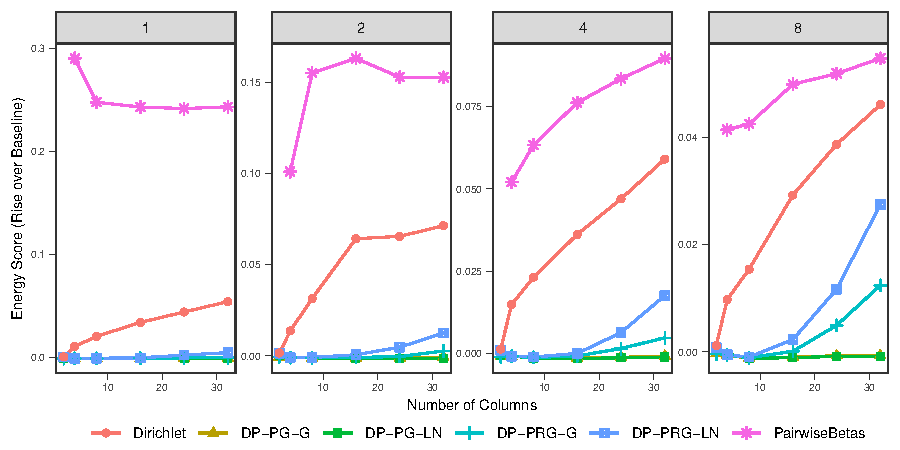
\includegraphics[height=3in, width = \textwidth]{./images/sim_es_rise}
\end{figure*}

\section{Data illustrations\label{sec:results}}
\hl{We apply the aforementioned models to simulated angular data. We then consider the analysis of atmospheric data. To tackle the difficult problem of assessing the convergence an MCMC chain for a large-dimensional model, we monitor the log-posterior density. In all the examples considered, MCMC samples produced stable traces of the log-posterior in less than 40 thousand  iterations. We use that as a burn-in, and thereafter sample 10 thousand additional iterations. We then thin the chain by retaining one every ten samples, to obtain 1000 total samples. These are used to generate samples from the posterior predictive densities. We used two different strategies to implement the MCMC samplers. For the models whose DP prior is centered around a log-normal distribution we used parallel tempering. This serves to overcome the very slow mixing that we observed for these cases. The temperature ladder was set as $t_s = 1.3^{s}$,  for $s \in \lbrace0,1,\ldots,5\rbrace$. This was set empirically in order to produce acceptable swap probabilities both for the simulated data, and real data. Parallel tempering produces chains with good mixing properties, but has a computational cost that  grows linearly with the number of temperatures. Thus, for the gamma-centered models, we used a single chain. We leverage the fast speed of each iteration, to obtain a large number of samples, that are appropriately thinned to deal with a mild autocorrelation. In summary, the strategy for log-normal centered models is based on a costly sampler with good mixing properties. The strategy for the gamma-centered models is based on a cheap sampler that can be run for a large number of iterations.}

\hl{Our hyperprior parameters are set as follows: for the gamma-centered models (PG--G, PRG--G), the shape parameter for the centering distribution~$\xi_{\ell}\sim \mathcal{G}\left(1,1\right)$, and rate parameter~$\tau_{\ell}\sim\mathcal{G}\left(2,2\right)$. For the log-normal centered models (PG--LN, PRG--LN), the centering distribution's log-mean $\bm{\mu}\sim\mathcal{N}_d\left(0,\bm{I}_d\right)$, and covariance matrix~$\Sigma\sim\mathcal{IW}\left(d + 10, (d+10)\bm{I}_{d}\right)$.  These values are intended such that draws from the prior for $\Sigma$ will weakly tend towards the identity matrix. For models learning rate parameters $\beta_{j\ell}$ (PG--G, PG--LN), the centering distribution's shape parameter $\zeta\sim\mathcal{G}\left(1,1\right)$ and rate parameter $\sigma\sim\mathcal{G}\left(2,2\right)$.  The choice of the $\mathcal{G}(2,2)$ for rate parameters places little mass near 0, in order to draw estimates for the value away from 0 for numerical stability.}

\subsection{Simulation Study\label{subsec:simulated}}
To evaluate our proposed approach for angular measure estimation we consider simulated datasets on $\mathbb{S}_{\infty}^{d-1}$, for values of $d$ ranging between \st{3 and 20}\hl{2 and 32}.  We generated each dataset as a mixture of \st{projected gammas}\hl{multivariate log-normal distributions, projected onto $\mathbb{S}_{\infty}^{d-1}$}\st{with the number of mixture components ranging between 3 and 12}. The generation procedure is detailed in Algorithm~\mbox{\ref{algo:simulated}}. \hl{We produced ten replicates of each configuration. We consider two gamma-centered and two log-normal centered DP mixture models, with and without restrictions in each case. To perform a comparative analysis we fitted the pairwise betas model proposed in\mbox{\cite{COOLEY2010}}}. 
\hl{We chose this model for comparison as it is implemented in the readily available package \mbox{\texttt{BMAmevt}} in R~\mbox{\citep{BMAmevt}}. \mbox{\texttt{BMAmevt}} provides samples from the predictive posterior distribution.}  
\hl{These are needed for the calculation of the energy scores that are at the basis of our comparison. In addition, \mbox{\texttt{BMAmevt}} can be fitted to moderately large multivariate observations.}
\hl{For the DP mixture models, the data are projected onto $\mathbb{S}_{10}^{d-1}$. For the other two models they are projected on $\mathbb{S}_1^{d-1}$.   We sampled each model for 50,000 iterations, dropping the first 40,000 as burn-in, and thinning to keep every 10th iteration after.  These settings were intended to provide a consistent sampling strategy that would work with every model, even if inefficient for some.}

\begin{algorithm}[ht]  % algorithm using algorithm package
\caption{Simulated Angular Dataset Generation Routine\label{algo:simulated}.
$\mu_j$, $\Sigma_j$ are the parameters of the mixture component distribution;
$\pi$ is the probability vector assigning weight mixture components; $\delta_i$
is the mixture component identifier for each simulated observation.}
\begin{algorithmic}
\For{$n_{\text{iter}}$ in $[1,\ldots,10]$}
\For{$n_{\text{mix}}$ in $[1, 2, 4, 8]$}
\For{$j$ in $1,\ldots,n_{\text{mix}}$}
\State Generate $\mu_{j} \sim \mathcal{N}_{32}\left(\bm{0},\bm{I}\right)$
\State Generate $\Sigma_{j}\sim\mathcal{IW}_{32}\left(70,70 \bm{I}\right)$
\EndFor
\State Generate $\pi\sim\text{Dirichlet}(\bm{10}_{n_{\text{mix}}})$
\For{$i$ in $1,\ldots,1000$}
\State Generate $\delta_i \sim \text{Categorical}(\pi)$
\State Generate $\bm{X}_i \sim \mathcal{LN}\left(\mu_{[\delta_i]},\Sigma_{[\delta_i]}\right)$
\EndFor
\For{$n_{\text{col}}$ in $[2,4,8,16,24,32]$}
\State Project columns 1 to $n_{\text{col}}$ of ${\bf X}$ onto $\mathcal{S}_{\infty}^{n_{\text{col}} - 1}$ and save.
\EndFor
\EndFor
\EndFor
\end{algorithmic}
\end{algorithm}

\st{Each one of the shape parameters $\alpha$ were generated $\alpha = \alpha_0 + \alpha_1$ where $\alpha_0 \sim \text{Unif}(\alpha_0\mid 0,4)$, $\alpha_1\sim \text{Gamma}(\alpha_1\mid 1,1)$.  The scale parameters $\beta$ were obtained as $\beta\sim\text{Unif}(\beta\mid 0.25, 2.5)$.}

\st{Figure~\mbox{\ref{fig:simpples}}, shows two sets of panels that illustrate the comparison between four different models used to fit the simulated data. We produced 16 different data sets, one for each of four different numbers of mixture components and four different dimensions. We considered three different models: DP mixtures of projected gamma; Projected restricted gamma; and projected restricted gamma with a multivariate log-normal prior. We calculated $S^\infty_{\text{PPL}}$ and $S_{\text{ES}}$ using predictive samples from each of fitted models. To provide a comparative baseline, we calculated the scores using samples generated directly using the same model and parameters that produced the simulated observations. The results are denoted as \emph{Gen} in the figure. We observe that the projected restricted Gamma model dominates in most situations, but the difference between projected restricted Gamma and the other gamma-based models tends to shrink as the number of dimensions increases. Alternatively, that difference appears to grow as the number of mixture components increases. The results from both scoring criteria are comparable.}

\hl{Figure~\mbox{\ref{fig:simpples}} shows the average rise over baseline in energy score as calculated on $\mathbb{S}_{\infty}^{d-1}$ using the kernel metric described in Proposition~\mbox{\ref{prop:rot}}, for models trained on simulated data.  After training a model, a posterior predictive dataset is generated, and the energy score is calculated as a Monte Carlo approximation of Equation~\mbox{\ref{eq:es}}.  In our analysis, after burn-in and thinning, we had 1,000 replicates from the posterior distribution, and generated 10 posterior predictive replicates per iteration. The \emph{baseline} value is the energy score of a new dataset from the same generating distribution as the training dataset, evaluated against the training dataset.  For the simulated data, we observe that the projected gamma models dominate the other two options considered, regardless of the choice of centering distribution.  The  projected restricted gamma models with a multivariate log-normal centering distribution appears to be dominated by the models based on the alternative centering distributions. Moreover, the performance deteriorates with the increase in dimensionality. Additionally, models centered around the log-normal distribution incur in the computational cost of multivariate normal evaluation and parallel tempering, taking approximately six times longer to sample relative to the gamma models.  We also note that the computational cost  of the pairwise betas model grows combinatorially, with a sample space of dimension $\binom{d}{2} + 1$. In our testing, \texttt{BMAmevt} is substantially faster than any of our proposed DP mixture models for low dimensions, however for examples with high number of dimensions, the computational time for \texttt{BMAmevt} was comparable or greater than that for DP-PG-G.  We compare computing times in our data analysis in Table~\mbox{\ref{tab:sampletime}}.}

\subsection{Integrated Vapor Transport\label{subsec:ivt}}
The \emph{integrated vapor transport} (IVT) is a two component vector that tracks the flow of the total water volume in a column of air over a given area \citep{ralph2017}.  IVT is increasingly used in the study of atmospheric rivers because of its direct relationship with orographically induced precipitation \citep{neiman2009water}. Atmospheric rivers (AR) are elongated areas of high local concentration of water vapor in the atmosphere that transport water from the tropics around the world. AR can cause extreme precipitation,  something that is usually associated with very large values of the IVT magnitude over a whole geographical area. In spite of this, AR are fundamental for the water supply of areas like California. Thus the importance of understanding the extreme behavior of IVT, including extreme tail dependence. We consider datasets that correspond to IVT estimated at two different spatial resolutions. The coarse resolution dataset is obtained from the European Centre for Medium-Range Weather Forecasts (ECMWF) Interim reanalysis (ERA-Interim) \citep{berrisford2011atmospheric,dee2011era}. The high resolution dataset corresponds to the latest ECMWF observational product, ERA5 \citep{hersbach2020era5}.

\begin{figure}[tb]
\caption{Grid cell locations for ERA-Interim (left) and ERA5 (right).\label{fig:gridlocs}}
\centering
\begin{minipage}{0.25\textwidth}
\centering
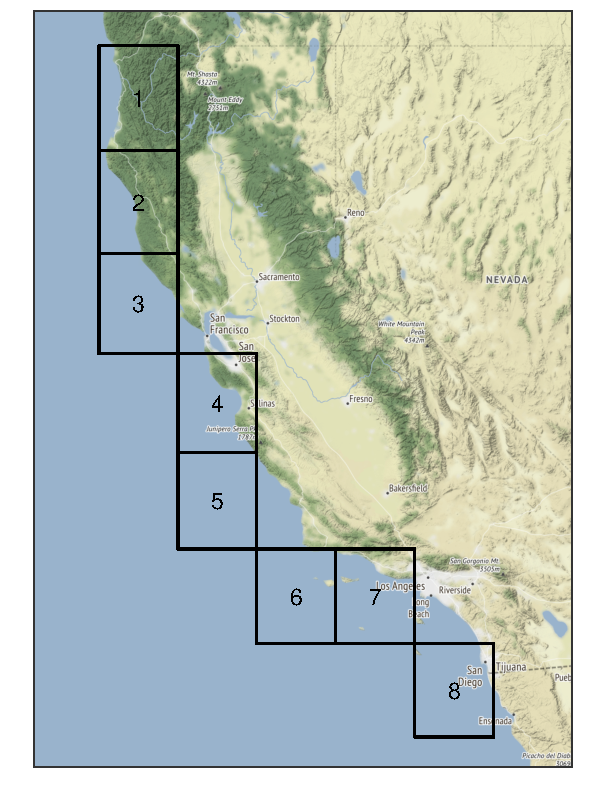
\includegraphics[width=0.99\linewidth]{./images/erai_grid}
\end{minipage}%
\begin{minipage}{0.25\textwidth}
\centering
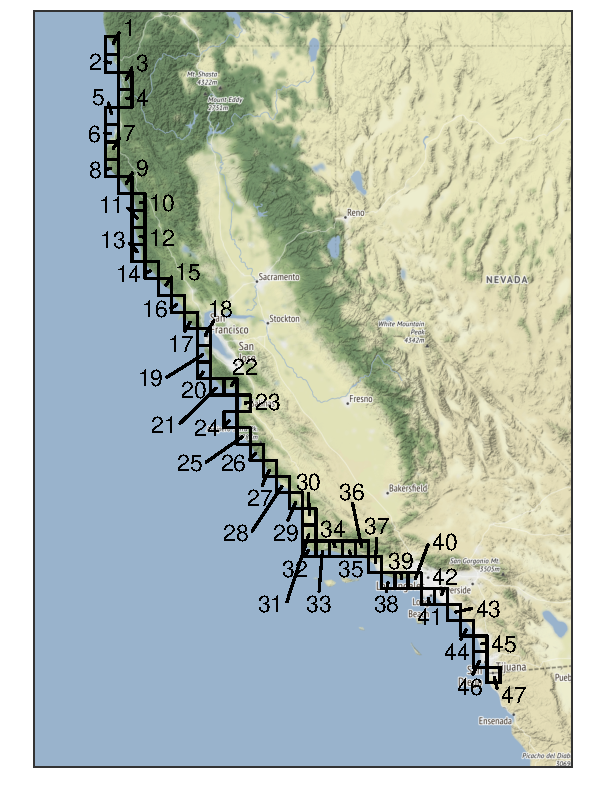
\includegraphics[width=0.99\linewidth]{./images/era5_grid}
\end{minipage}
\end{figure}

Our data correspond to daily average values for the IVT magnitude along the coast of California.  The ERA-Interim data used covers the time period 1979 through 2014 (37 years) omitting leap days, and eight grid cells that correspond to the coast of California.  The ERA5 data cover the time period 1979 through 2019 (42 years) with the same restriction, and  47 grid cells for the coast of California.  This gives us the opportunity to illustrate the performance of our method in multivariate settings of very different dimensions. Figure~\ref{fig:gridlocs} provides a visual representation of the area these grid cells \st{represent}\hl{cover}.

\begin{algorithm}[htb]
\caption{Data preprocessing to isolate and transform data exhibiting extreme behavior.  $r_i$ represents the radial component, and $\bm{v}_i$ the angular component.  The declustering portion is relevant for data correlated in time.\label{algo:processing}}
\begin{algorithmic}
\For{$\ell = 1,\ldots,d$}
\State Set $b_{t,\ell} = \hat{F}_{\ell}^{-1}\left(1 - \frac{1}{t}\right)$.
\State With $\bm{ x}_{\ell} > b_{t,\ell}$, fit $a_{\ell}$, $\xi_{\ell}$ via MLE according to generalized Pareto likelihood.
\EndFor
\For{$i = 1,\ldots,n$}
\State Define $z_{i,\ell} = \left(1 + \xi_{\ell}\frac{x_{i,\ell} - b_{t,\ell}}{a_{\ell}}\right)_{+}^{1/\xi_{\ell}}$; $\;\;\;$ then $r_i = \pnorm{\bm{ z}_i}{\infty}$, $\;\;\bm{ v}_i = \frac{\bm{ z}_i}{\pnorm{\bm{ z}_i}{\infty}}$
\EndFor
\State Subset $\bm{ r},\bm{ v}$ such that $r_i \geq 1$
\If{declustering}
\For{$i = 1,\ldots,n$}
\State If $r_i \geq 1$ and $r_{i-1} \geq 1$, drop the lesser (and associated $v_i$) from data set.
\EndFor
\EndIf
\end{algorithmic}
\end{algorithm}

\begin{figure*}[ht]%{l}{0.45\textwidth}
\centering
\caption{Pairwise plots from ERA-Interim data after transformation and projection to ${\mathbb S}_{\infty}^{7}$.  Down the diagonal are marginal kernel densities, with two-dimensional histograms on the off-diagonal.  In those plots, red indicates a higher density.  All data is between 0 and 1.\label{fig:erai_data}}
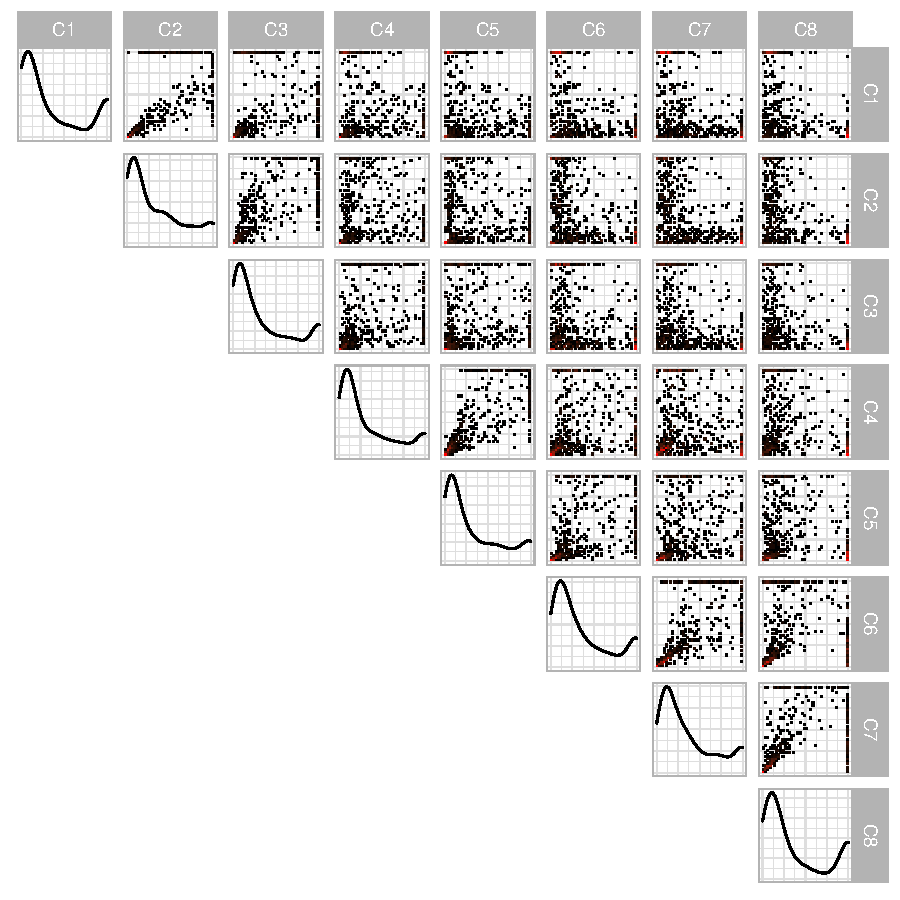
\includegraphics[width=.7\linewidth]{./images/data_transformed}
\end{figure*}

Fitting our models to the IVT data requires some pre-processing. First, we subset the data to the rainy season, which in California runs roughly from November to March.  Following the approach described in Section \ref{sec:methodology} we estimate the shape and scale parameters of a univariate GP, in each dimension, using maximum likelihood. We set the threshold in each dimensions $\ell$ as $b_{t,\ell} = \hat{F}_{\ell}^{-1}(1 - t^{-1})$, where $\hat{F}$ is the empirical CDF and $t=20$, that corresponds to the $95$ percentile. We then use the transformation in Equation \eqref{eqn:standardization} to standardize the observations.  Dividing each standardized observation by its $\mathcal{L}_{\infty}$ norm, we obtain a projection onto $\mathcal{S}_{\infty}^{d-1}$. As the data correspond to a daily time series, the observations are temporally correlated.  For each group of consecutive standardized vectors $z_i$ such  that  $\inorm{z_i} > 1$, we retain only the vector with the largest $\mathcal{L}_{\infty}$ norm.  The complete procedure is outlined in Algorithm~\ref{algo:processing}.

After subsetting the ERA-Interim data to the rainy season we have $5587$ observations. After the processing and declustering described in Algorithm~\ref{algo:processing}, this number reduces to $511$ observations. A pairwise plot of the transformed data after processing and declustering is presented in Figure~\ref{fig:erai_data}.  From this, we note that the marginal densities display strong similarities, with a large spike near 0 and a small spike near 1. A value of 1 in a particular axis indicates that the standardized threshold exceedance was largest in that dimension.  The off-diagonal plots correspond to pairwise density plots.  We observe that some site pairs, such as $(1,2)$, $(7,8)$, and especially $(4,5)$ have the bulk of their data concentrated in a small arc along the $45^{\circ}$, while other site combinations such as $(3,6)$, $(2,7)$, or $(1,8)$ the data is split, favoring one side or the other of the $45^{\circ}$ line. For the ERA5 data, after subsetting we have $6342$ observations, which reduces to $532$ observations after processing and declustering. We fit the PG--G, PRG--G, PG--LN, and PRG--LN models to both datasets.

\begin{table}[htb]
\centering
\caption{Energy score criterion from fitted models against the IVT data. Lower is better.\label{tab:dev}}
\newlength{\templen}
\setlength\templen{\tabcolsep}
\setlength\tabcolsep{3.5pt}
\begin{tabular}{c|ccccc}
\toprule
Source & \begin{tabular}{@{}c@{}}Pairwise \\ Betas\end{tabular} & PG-G & PG-LN & PRG-G & PRG-LN\\
\midrule
\begin{tabular}{@{}c@{}}ERA- \\ Interim\end{tabular} & $0.8620$ & $0.8003$ & $0.7986$ & $\bm{0.7966}$ & $0.7970$\\
ERA5 & $2.0311$ & $1.6404$ & $1.5576$ & $\bm{1.4349}$ & $1.5051$\\
\bottomrule
\end{tabular}
\setlength\tabcolsep{\templen}
\end{table}

\begin{table}[htb]
\centering
\caption{Time to sample (in minutes) 50,000 iterations for various models\label{tab:sampletime}}
\setlength\templen{\tabcolsep}
\setlength\tabcolsep{3.5pt}
\begin{tabular}{c|ccccc}
\toprule
Source & \begin{tabular}{@{}c@{}}Pairwise \\ Betas\end{tabular} & PG-G & PG-LN & PRG-G & PRG-LN\\
\midrule
\begin{tabular}{@{}c@{}}ERA- \\ Interim\end{tabular} & $1.5$ & $16.3$ & $66.5$ & $14.8$ & $52.9$\\
ERA5 & $53.1$ & $19.4$ & $153.4$ & $24.6$ & $121.4$\\
\bottomrule
\end{tabular}
\setlength\tabcolsep{\templen}
\end{table}

Table~\ref{tab:dev} shows the values of the estimated \st{posterior predictive loss and }energy scores for the different models considered. We observe that, \st{as in}\hl{contrary to} the \st{case of}\hl{results in} the simulation study \st{shown} in Figure\st{s}~\ref{fig:simpples}, the preferred model is the projected restricted gamma models{\st .  Penalization for the unrestricted gamma model is stronger for the real data than for the simulated data. We also observe that the restricted gamma model with the log-normal prior performs significantly better than the restricted gamma model with the gamma prior on the higher dimensional data. This is the opposite of the result obtained in the simulation example.}{\hl, though for the lower-dimensional ERA-Interim data, all models perform comparably.  Table~\ref{tab:sampletime} shows the computing times needed to fit the different models to the two datasets.  We see the effect of dimensionality on the various models; for gamma centered models it grows linearly; for the log--normal centered model, it will grow superlinearly as matrix inversion becomes the most costly operation.  For \texttt{BMAmevt}, its parameter space grows combinatorically with the number of dimensions, and thus so does computational complexity and sampling time.}

\begin{figure*}[htb]
\centering
\caption{Pairwise extremal dependence coefficients for IVT data using the PRG--G model.\label{fig:chi_ij}}
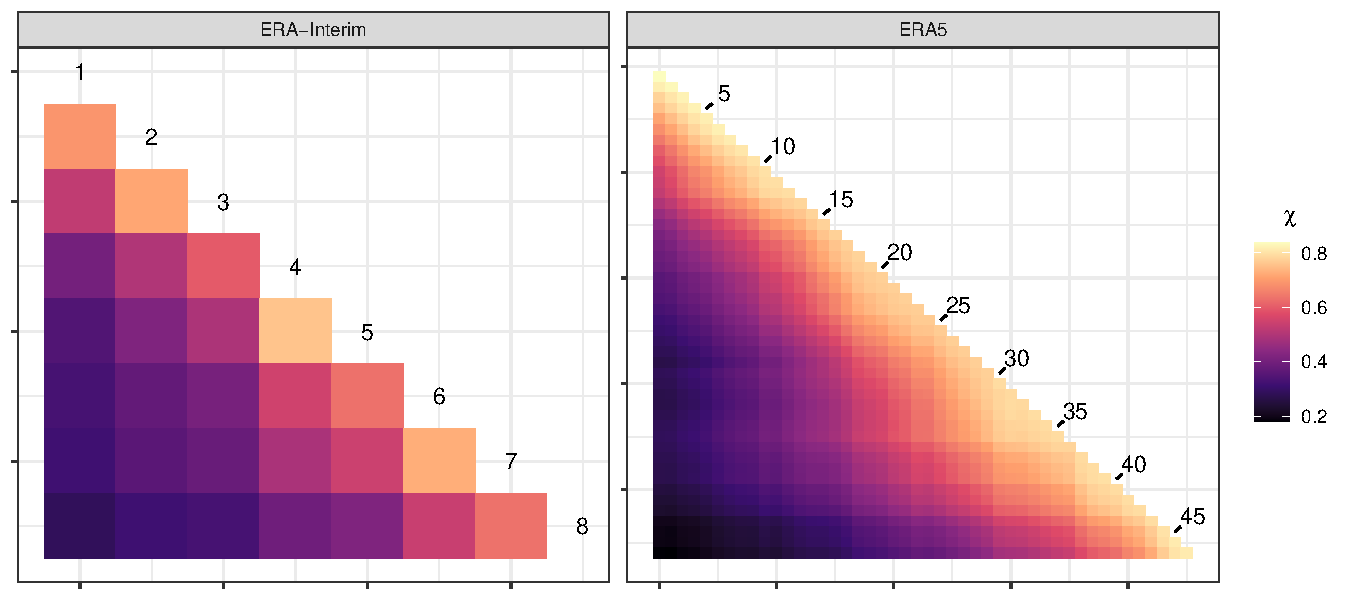
\includegraphics[width=0.9\textwidth]{./images/chi_ij_c}
\end{figure*}

We consider an exploration of the pairwise extremal dependence using Monte Carlo estimates of the coefficients in  Equation~\ref{eqn:chi_ij}. For this we use samples obtained from the PRG--G model. Figure~\ref{fig:chi_ij} provides a graphical analysis of the results. The coefficients achieve values between $0.286$ and $0.759$ for the ERA-Interim data and between $0.181$ and $0.840$ for the ERA5 data.  The greater range in dependence scores observed with the ERA5 data versus ERA-Interim speaks to the greater granularity of the ERA5 data\st{--}\hl{, indicating that }distance between locations is a strong contributor to the strength of the pairwise asymptotic dependence. The highest coefficients are $0.759$ for locations 4 and 5 in the ERA-Interim data and $0.840$ for locations 1 and 2 in the ERA5 data.  Clearly, pairwise asymptotic dependence coefficients tell a limited story, as a particular dependence may include more than two locations.   We can, however, glean some information from the patterns that emerge in two dimensions.  For the ERA-Interim data, we observe a possible cluster between cells 5-8, indicating a strong dependence among these cells.  Analogously, for the ERA5 data, we observe three possible groups of locations.

\begin{figure*}[htb]
\centering
\caption{Conditional survival curves for selected locations, using ERA-Interim, and PRG-G model,  conditioning on all other dimensions at greater than 90th percentile (fitted)\label{fig:condsurv1d}. The left panel uses original units. Right panel uses standardized units.}
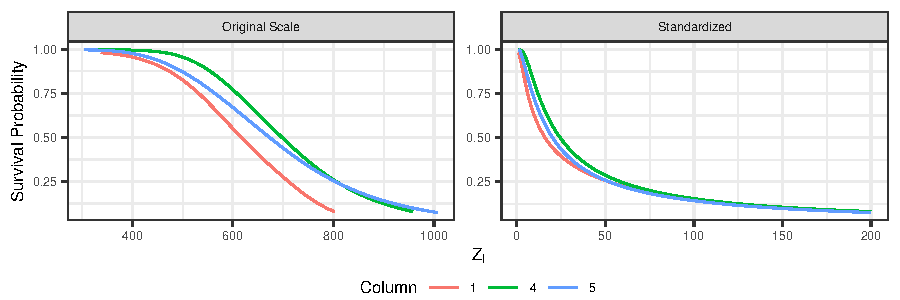
\includegraphics[width=\linewidth]{./images/condsurv_1d}
\end{figure*}

\begin{figure*}[htb]
\centering
\caption{Pairwise conditional survival curves for selected locations, using
ERA-Interim, and PRG-G model, conditioning on all other dimensions at greater
than 90th percentile (fitted).\label{fig:condsurv2d}}
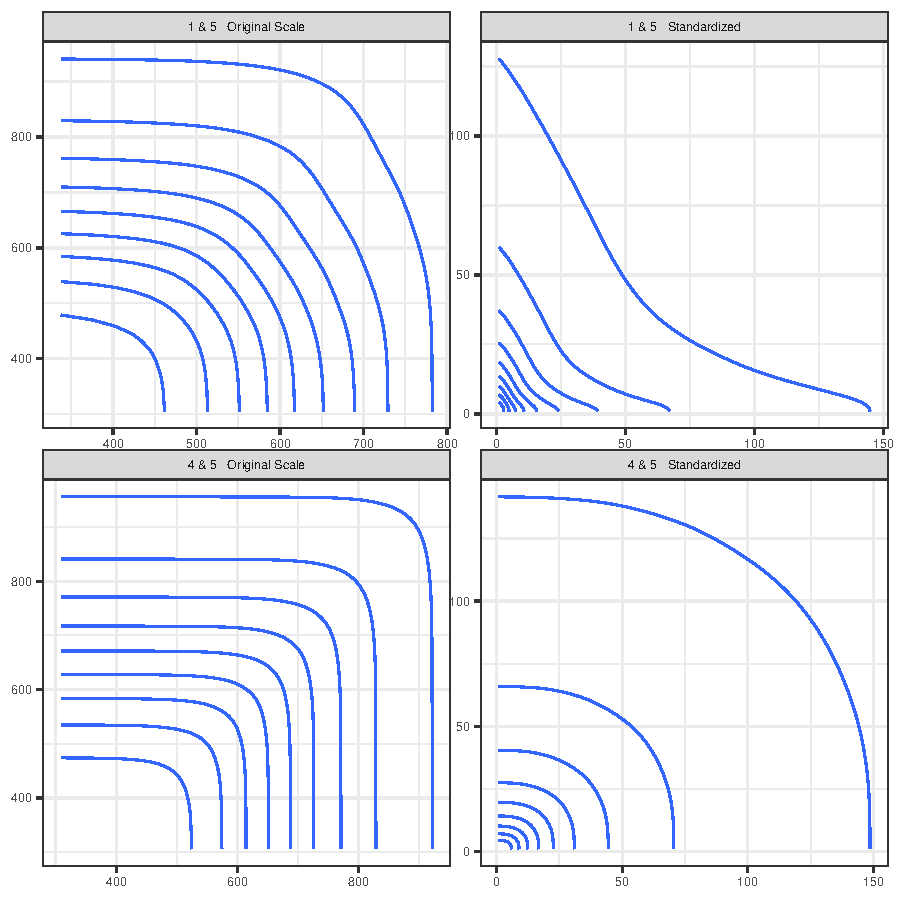
\includegraphics[height=4in, width=4in]{./images/condsurv_2d}
\end{figure*}

Figure~\ref{fig:condsurv1d} shows, for the ERA-Interim data under the PRG--G model, the conditional survival curve defined in Equation~\ref{eqn:condsurv}, for one dimension, conditioned on all other dimensions being greater than their (fitted) $90$th percentile.  Figure~\ref{fig:condsurv2d} presents the bi-variate conditional survival function, conditioning on all other dimensions.  These results illustrate quantitatively how extremal dependence affects the shape of the conditional survival curves.  The two top panels represent the joint survival function between grid locations 4 and 5, which are shown in Figure~\ref{fig:chi_ij} to exhibit strong  extremal dependence.  We observe that the joint survival surface is strongly convex.  The bottom panels represent the joint survival surface between grid locations 1 and 5, which exhibited low extremal dependence.  In this case the shape of the contours tend to be concave, quite different from the shapes observed in the top panels.

Using our proposed scoring criteria, we explored the effect of the choice of $p$ on the final results. Using the simulated data, generated from a mixture of projected Gammas, we were unable to observe sizeable differences in the scores for $p$ ranging between 1 and 15.   However, for the IVT data, we observed a drop in the energy score associated with higher $p$, with diminishing effect as $p$ increased.  We observed no significant differences in the performance of the model that uses $p=10$, which corresponds to the analysis presented, relative to the one that uses $p=15$.


\section{Conclusion\label{sec:conclusion}}
In this paper, we have built upon the definition of the multivariate Pareto described in \cite{ferreira2014} to establish a useful representation of its dependence structure, through the distribution of its angular component, which is supported on the positive orthant of the unit hypersphere under the $\mathcal{L}_{\infty}$ norm.  Due to the inherent difficulty of obtaining \st{a}\hl{the likelihood of} distribution\hl{s} with support on ${\mathbb S}^{d-1}_\infty$ our method \st{projects distributions, supported on the positive quadrant and based on products of independent gammas,  onto the manifold ${\mathbb S}_{p}^{d-1}$. Samples of the resulting probability distribution are then projected onto ${\mathbb S}_{\infty}^{d-1}$. }\hl{transforms the data to ${\mathbb S}_{p}^{d-1}$, fits then using mixtures of products of independent gammas, then transforms the predictions back to ${\mathbb S}^{d-1}_\infty$.} As ${\mathbb S}_{p}^{d-1}$ converges to ${\mathbb S}_{\infty}^{d-1}$ as  $p\to\infty$, we expect the \hl{proposed }resampling to be efficient for large enough $p$. In fact, our exploration of the simulated and real data indicates that the procedure is robust to the choice of moderately large values of $p$. \hl{Our method includes two inferential steps. The first consists of the estimation of the marginal Pareto distributions. The second consists of the estimation of the angular density. Parameter uncertainty incurred in the former is not propagated to the latter. Conceptually, an integrated approach that accounts for all the estimation uncertainty is conceivable. Unfortunately, this leads to posterior distributions with complex data dependent restrictions that are very difficult to explore, especially in large dimensional settings. In fact, our attempts to fit a simple parametric model for the marginals and the angular measure jointly in several dimensions were not successful.}

\st{We explored the behavior of the proposed model using simulated data from mixtures of projected Gammas with varying degrees of complexity---both in terms of dimensionality and in number of mixture components.  From this, we learned that the additional flexibility offered by varying the $\beta$ term---the rate parameter of the Gamma distribution---does not result in increased model fidelity in a mixture setting.  Within the tested range, between 3 and 20 dimensions, we observed that the additional information provided by a log--normal centering distribution did not translate to additional model fidelity.  However, for real data, with 47 dimensions, we did observe an effect.}

\hl{In this paper we have focused on a particular representation of the multivariate Pareto distribution for PoT inference on extreme values. To this end, our model  provides a computationally efficient and flexible approach. An interesting extension of the proposed model is to consider regressions of extreme value responses, due to extreme value inputs following the ideas in  \mbox{\cite{carvalho2022}}. This will produce PoT based Bayesian non-parametric extreme value regression models. More generally,  models that allow for covariate-dependent extremal dependence \mbox{\citep{mhalla2019}} could be considered. In addition, we notice that our approach is based on flexibly  modeling angular distributions for any $p$-norm. As such, it can be applied to other problems focused on high dimensional directional statistics constrained to a cone of directions.}

The computations in this paper were performed on a desktop computer with an AMD Ryzen 5950X processor. The program is largely single-threaded, so computation time is not dependent on available core count.  In each case, we run the MCMC chain for 50\,000 iterations, with a burn-in of 40\,000 samples.  Fitting the PG--G model on the ERA5 dataset took approximately 15 minutes.  Work is in progress to optimize the code, and explore parallelization where possible.  We are also exploring alternative computational approaches that will make it feasible to tackle very high dimensional problems, such as variational Bayes. In fact, to elaborate on the study of IVT, there is a need to consider several hundreds, if not thousands, of grid cells over the Pacific Ocean in order to obtain a good description of atmospheric  events responsible for large storm activity over California.

\section*{Acknowledgements}
This material is based upon work supported by the National Science Foundation under Grant No. SES-2050012 and DMS-2153277.

\bibliography{./refs}

\end{document}

% EOF
